%% bare_conf_compsoc.tex
%% V1.4b
%% 2015/08/26
%% by Michael Shell && Semih Can Karakoc
%% See:
%% http://www.michaelshell.org/
%% for current contact information.
%%
%% This is a skeleton file demonstrating the use of IEEEtran.cls
%% (requires IEEEtran.cls version 1.8b or later) with an IEEE Computer
%% Society conference paper.
%%
%% Support sites:
%% http://www.michaelshell.org/tex/ieeetran/
%% http://www.ctan.org/pkg/ieeetran
%% and
%% http://www.ieee.org/

%%*************************************************************************
%% Legal Notice:
%% This code is offered as-is without any warranty either expressed or
%% implied; without even the implied warranty of MERCHANTABILITY or
%% FITNESS FOR A PARTICULAR PURPOSE! 
%% User assumes all risk.
%% In no event shall the IEEE or any contributor to this code be liable for
%% any damages or losses, including, but not limited to, incidental,
%% consequential, or any other damages, resulting from the use or misuse
%% of any information contained here.
%%
%% All comments are the opinions of their respective authors and are not
%% necessarily endorsed by the IEEE.
%%
%% This work is distributed under the LaTeX Project Public License (LPPL)
%% ( http://www.latex-project.org/ ) version 1.3, and may be freely used,
%% distributed and modified. A copy of the LPPL, version 1.3, is included
%% in the base LaTeX documentation of all distributions of LaTeX released
%% 2003/12/01 or later.
%% Retain all contribution notices and credits.
%% ** Modified files should be clearly indicated as such, including  **
%% ** renaming them and changing author support contact information. **
%%*************************************************************************


% *** Authors should verify (and, if needed, correct) their LaTeX system  ***
% *** with the testflow diagnostic prior to trusting their LaTeX platform ***
% *** with production work. The IEEE's font choices and paper sizes can   ***
% *** trigger bugs that do not appear when using other class files.       ***                          ***
% The testflow support page is at:
% http://www.michaelshell.org/tex/testflow/


\documentclass[conference,%compsoc%
]{IEEEtran}
% Some/most Computer Society conferences require the compsoc mode option,
% but others may want the standard conference format.
\IEEEoverridecommandlockouts
% If IEEEtran.cls has not been installed into the LaTeX system files,
% manually specify the path to it like:
% \documentclass[conference,compsoc]{../sty/IEEEtran}

\usepackage[dutch]{babel}
\usepackage[colorlinks=true, allcolors=blue]{hyperref}
\usepackage{parskip}
% More defined colors
\usepackage{enumitem}
\usepackage[dvipsnames]{xcolor}
\usepackage{amsmath,amssymb,amsfonts}
\usepackage{algorithmic}
\usepackage[ruled,vlined]{algorithm2e}
\usepackage{pifont}
% The preceding line is only needed to identify funding in the first footnote. If that is unneeded, please comment it out.
\usepackage{textcomp}
\usepackage{listings}
 % More defined colors
\usepackage[american voltages,siunitx]{circuitikz}
\usepackage{xcolor}
\usepackage{cite}

\definecolor{codegreen}{rgb}{0,0.6,0}
\definecolor{codegray}{rgb}{0.5,0.5,0.5}
\definecolor{codepurple}{rgb}{0.58,0,0.82}
\definecolor{backcolour}{rgb}{0.95,0.95,0.92}

\lstdefinelanguage{JavaScript}{
  keywords={break, case, catch, continue, debugger, default, delete, do, else, false, finally, for, function, if, in, instanceof, new, null, return, switch, this, throw, true, try, typeof, var, void, while, with},
  ndkeywords={class, export, boolean, throw, implements, import, this, setTimeout, reload},
  ndkeywordstyle=\color{pink}\bfseries,
  backgroundcolor=\color{backcolour},  
  comment=[l]{//}, 
  commentstyle=\color{codegreen},
  keywordstyle=\color{blue},
  numberstyle=\tiny\color{codegray},
  stringstyle=\color{codepurple},
  basicstyle=\ttfamily\footnotesize,
  breakatwhitespace=false,         
  breaklines=true,                 
  captionpos=b,                    
  keepspaces=true,                 
  numbers=left,                    
  numbersep=5pt,                  
  showspaces=false,                
  showstringspaces=false,
  showtabs=false,                  
  tabsize=2
}
\lstset{ %
  language=C,                            % choose the language of the code
  basicstyle=\footnotesize,              % the size of the fonts that are used for the code
  backgroundcolor=\color{White},         % choose the background color. You must add \usepackage{color}
  commentstyle=\color{help}\textit,
  keywordstyle=\color{keyword}\textbf,
  breaklines=true,                       % sets automatic line breaking
  breakatwhitespace=true,                % sets if automatic breaks should only happen at whitespace
  showspaces=false,                      % show spaces adding particular underscores
  showstringspaces=true,                 % underline spaces within strings
  showtabs=true,                         % show tabs within strings adding particular underscores
  frame=none,                              % adds a frame around the code - none, single
  tabsize=8,                             % sets default tabsize to 8 spaces
  captionpos=b,                          % sets the caption-position to bottom
  numbers=left,                          % where to put the line-numbers -none, left, right
  numberstyle=\footnotesize,             % the size of the fonts that are used for the line-numbers
  stepnumber=1,                          % the step between two line-numbers. If it's 1 each line
                                         % will be numbered
}
\lstdefinestyle{mystyle}{
    backgroundcolor=\color{backcolour},   
    commentstyle=\color{codegreen},
    keywordstyle=\color{magenta},
    numberstyle=\tiny\color{codegray},
    stringstyle=\color{codepurple},
    basicstyle=\ttfamily\footnotesize,
    breakatwhitespace=false,         
    breaklines=true,                 
    captionpos=b,                    
    keepspaces=true,                 
    numbers=left,                    
    numbersep=5pt,                  
    showspaces=false,                
    showstringspaces=false,
    showtabs=false,                  
    tabsize=2
}

\lstset{style=mystyle}

% Some very useful LaTeX packages include:
% (uncomment the ones you want to load)


% *** MISC UTILITY PACKAGES ***
%
%\usepackage{ifpdf}
% Heiko Oberdiek's ifpdf.sty is very useful if you need conditional
% compilation based on whether the output is pdf or dvi.
% usage:
% \ifpdf
%   % pdf code
% \else
%   % dvi code
% \fi
% The latest version of ifpdf.sty can be obtained from:
% http://www.ctan.org/pkg/ifpdf
% Also, note that IEEEtran.cls V1.7 and later provides a builtin
% \ifCLASSINFOpdf conditional that works the same way.
% When switching from latex to pdflatex and vice-versa, the compiler may
% have to be run twice to clear warning/error messages.
 






% *** CITATION PACKAGES ***
%
\ifCLASSOPTIONcompsoc
  % IEEE Computer Society needs nocompress option
  % requires cite.sty v4.0 or later (November 2003)
  \usepackage[nocompress]{cite}
\else
  % normal IEEE
  \usepackage{cite}
\fi
% cite.sty was written by Donald Arseneau
% V1.6 and later of IEEEtran pre-defines the format of the cite.sty package
% \cite{} output to follow that of the IEEE. Loading the cite package will
% result in citation numbers being automatically sorted and properly
% "compressed/ranged". e.g., [1], [9], [2], [7], [5], [6] without using
% cite.sty will become [1], [2], [5]--[7], [9] using cite.sty. cite.sty's
% \cite will automatically add leading space, if needed. Use cite.sty's
% noadjust option (cite.sty V3.8 and later) if you want to turn this off
% such as if a citation ever needs to be enclosed in parenthesis.
% cite.sty is already installed on most LaTeX systems. Be sure and use
% version 5.0 (2009-03-20) and later if using hyperref.sty.
% The latest version can be obtained at:
% http://www.ctan.org/pkg/cite
% The documentation is contained in the cite.sty file itself.
%
% Note that some packages require special options to format as the Computer
% Society requires. In particular, Computer Society  papers do not use
% compressed citation ranges as is done in typical IEEE papers
% (e.g., [1]-[4]). Instead, they list every citation separately in order
% (e.g., [1], [2], [3], [4]). To get the latter we need to load the cite
% package with the nocompress option which is supported by cite.sty v4.0
% and later.





% *** GRAPHICS RELATED PACKAGES ***
%
\ifCLASSINFOpdf
  \usepackage[]{graphicx} 
  %pdftex
  % declare the path(s) where your graphic files are
  % \graphicspath{{../pdf/}{../jpeg/}}
  \graphicspath{ {./Images/} }
  % and their extensions so you won't have to specify these with
  % every instance of \includegraphics
   \DeclareGraphicsExtensions{.pdf,.jpeg,.png}
\else
  % or other class option (dvipsone, dvipdf, if not using dvips). graphicx
  % will default to the driver specified in the system graphics.cfg if no
  % driver is specified.
  % \usepackage[dvips]{graphicx}
  % declare the path(s) where your graphic files are
  % \graphicspath{{../eps/}}
  % and their extensions so you won't have to specify these with
  % every instance of \includegraphics
  % \DeclareGraphicsExtensions{.eps}
\fi
% graphicx was written by David Carlisle and Sebastian Rahtz. It is
% required if you want graphics, photos, etc. graphicx.sty is already
% installed on most LaTeX systems. The latest version and documentation
% can be obtained at: 
% http://www.ctan.org/pkg/graphicx
% Another good source of documentation is "Using Imported Graphics in
% LaTeX2e" by Keith Reckdahl which can be found at:
% http://www.ctan.org/pkg/epslatex
%
% latex, and pdflatex in dvi mode, support graphics in encapsulated
% postscript (.eps) format. pdflatex in pdf mode supports graphics
% in .pdf, .jpeg, .png and .mps (metapost) formats. Users should ensure
% that all non-photo figures use a vector format (.eps, .pdf, .mps) and
% not a bitmapped formats (.jpeg, .png). The IEEE frowns on bitmapped formats
% which can result in "jaggedy"/blurry rendering of lines and letters as
% well as large increases in file sizes.
%
% You can find documentation about the pdfTeX application at:
% http://www.tug.org/applications/pdftex





% *** MATH PACKAGES ***
%
%\usepackage{amsmath}
% A popular package from the American Mathematical Society that provides
% many useful and powerful commands for dealing with mathematics.
%
% Note that the amsmath package sets \interdisplaylinepenalty to 10000
% thus preventing page breaks from occurring within multiline equations. Use:
%\interdisplaylinepenalty=2500
% after loading amsmath to restore such page breaks as IEEEtran.cls normally
% does. amsmath.sty is already installed on most LaTeX systems. The latest
% version and documentation can be obtained at:
% http://www.ctan.org/pkg/amsmath





% *** SPECIALIZED LIST PACKAGES ***
%
%\usepackage{algorithmic}
% algorithmic.sty was written by Peter Williams and Rogerio Brito.
% This package provides an algorithmic environment fo describing algorithms.
% You can use the algorithmic environment in-text or within a figure
% environment to provide for a floating algorithm. Do NOT use the algorithm
% floating environment provided by algorithm.sty (by the same authors) or
% algorithm2e.sty (by Christophe Fiorio) as the IEEE does not use dedicated
% algorithm float types and packages that provide these will not provide
% correct IEEE style captions. The latest version and documentation of
% algorithmic.sty can be obtained at:
% http://www.ctan.org/pkg/algorithms
% Also of interest may be the (relatively newer and more customizable)
% algorithmicx.sty package by Szasz Janos:
% http://www.ctan.org/pkg/algorithmicx




% *** ALIGNMENT PACKAGES ***
%
%\usepackage{array}
% Frank Mittelbach's and David Carlisle's array.sty patches and improves
% the standard LaTeX2e array and tabular environments to provide better
% appearance and additional user controls. As the default LaTeX2e table
% generation code is lacking to the point of almost being broken with
% respect to the quality of the end results, all users are strongly
% advised to use an enhanced (at the very least that provided by array.sty)
% set of table tools. array.sty is already installed on most systems. The
% latest version and documentation can be obtained at:
% http://www.ctan.org/pkg/array


% IEEEtran contains the IEEEeqnarray family of commands that can be used to
% generate multiline equations as well as matrices, tables, etc., of high
% quality.




% *** SUBFIGURE PACKAGES ***
%\ifCLASSOPTIONcompsoc
%  \usepackage[caption=false,font=footnotesize,labelfont=sf,textfont=sf]{subfig}
%\else
%  \usepackage[caption=false,font=footnotesize]{subfig}
%\fi
% subfig.sty, written by Steven Douglas Cochran, is the modern replacement
% for subfigure.sty, the latter of which is no longer maintained and is
% incompatible with some LaTeX packages including fixltx2e. However,
% subfig.sty requires and automatically loads Axel Sommerfeldt's caption.sty
% which will override IEEEtran.cls' handling of captions and this will result
% in non-IEEE style figure/table captions. To prevent this problem, be sure
% and invoke subfig.sty's "caption=false" package option (available since
% subfig.sty version 1.3, 2005/06/28) as this is will preserve IEEEtran.cls
% handling of captions.
% Note that the Computer Society format requires a sans serif font rather
% than the serif font used in traditional IEEE formatting and thus the need
% to invoke different subfig.sty package options depending on whether
% compsoc mode has been enabled.
%
% The latest version and documentation of subfig.sty can be obtained at:
% http://www.ctan.org/pkg/subfig




% *** FLOAT PACKAGES ***
%
%\usepackage{fixltx2e}
% fixltx2e, the successor to the earlier fix2col.sty, was written by
% Frank Mittelbach and David Carlisle. This package corrects a few problems
% in the LaTeX2e kernel, the most notable of which is that in current
% LaTeX2e releases, the ordering of single and double column floats is not
% guaranteed to be preserved. Thus, an unpatched LaTeX2e can allow a
% single column figure to be placed prior to an earlier double column
% figure.
% Be aware that LaTeX2e kernels dated 2015 and later have fixltx2e.sty's
% corrections already built into the system in which case a warning will
% be issued if an attempt is made to load fixltx2e.sty as it is no longer
% needed.
% The latest version and documentation can be found at:
% http://www.ctan.org/pkg/fixltx2e


%\usepackage{stfloats}
% stfloats.sty was written by Sigitas Tolusis. This package gives LaTeX2e
% the ability to do double column floats at the bottom of the page as well
% as the top. (e.g., "\begin{figure*}[!b]" is not normally possible in
% LaTeX2e). It also provides a command:
%\fnbelowfloat
% to enable the placement of footnotes below bottom floats (the standard
% LaTeX2e kernel puts them above bottom floats). This is an invasive package
% which rewrites many portions of the LaTeX2e float routines. It may not work
% with other packages that modify the LaTeX2e float routines. The latest
% version and documentation can be obtained at:
% http://www.ctan.org/pkg/stfloats
% Do not use the stfloats baselinefloat ability as the IEEE does not allow
% \baselineskip to stretch. Authors submitting work to the IEEE should note
% that the IEEE rarely uses double column equations and that authors should try
% to avoid such use. Do not be tempted to use the cuted.sty or midfloat.sty
% packages (also by Sigitas Tolusis) as the IEEE does not format its papers in
% such ways.
% Do not attempt to use stfloats with fixltx2e as they are incompatible.
% Instead, use Morten Hogholm'a dblfloatfix which combines the features
% of both fixltx2e and stfloats:
%
% \usepackage{dblfloatfix}
% The latest version can be found at:
% http://www.ctan.org/pkg/dblfloatfix




% *** PDF, URL AND HYPERLINK PACKAGES ***
%
%\usepackage{url}
% url.sty was written by Donald Arseneau. It provides better support for
% handling and breaking URLs. url.sty is already installed on most LaTeX
% systems. The latest version and documentation can be obtained at:
% http://www.ctan.org/pkg/url
% Basically, \url{my_url_here}.




% *** Do not adjust lengths that control margins, column widths, etc. ***
% *** Do not use packages that alter fonts (such as pslatex).         ***
% There should be no need to do such things with IEEEtran.cls V1.6 and later.
% (Unless specifically asked to do so by the journal or conference you plan
% to submit to, of course. )


% correct bad hyphenation here
\hyphenation{op-tical net-works semi-conduc-tor}


\begin{document}
%
% paper title
% Titles are generally capitalized except for words such as a, an, and, as,
% at, but, by, for, in, nor, of, on, or, the, to and up, which are usually
% not capitalized unless they are the first or last word of the title.
% Linebreaks \\ can be used within to get better formatting as desired.
% Do not put math or special symbols in the title.
\title{Hard- en Software Ontwerp van Webinterface dat Temperatuur en Luchtvochtigheid \textit{Realtime} Presenteert}
%Electrical Design of Tetris Game based on a Single Chip Microcontroller

% author names and affiliations
% use a multiple column layout for up to three different
% affiliations
\author{\IEEEauthorblockN{Semih C Karakoç}
\IEEEauthorblockA{\textit{Computer Science and Engineering}\\
Inholland University of Applied Sciences\\
Alkmaar, Netherlands\\
Email: 695258@student.inholland.nl}}
% \and
% \IEEEauthorblockN{Homer Simpson}
% \IEEEauthorblockA{Twentieth Century Fox\\
% Springfield, USA\\
% Email: homer@thesimpsons.com}
% \and
% \IEEEauthorblockN{James Kirk\\ and Montgomery Scott}
% \IEEEauthorblockA{Starfleet Academy\\
% San Francisco, California 96678-2391\\
% Telephone: (800) 555--1212\\
% Fax: (888) 555--1212}}

% conference papers do not typically use \thanks and this command
% is locked out in conference mode. If really needed, such as for
% the acknowledgment of grants, issue a \IEEEoverridecommandlockouts
% after \documentclass

% for over three affiliations, or if they all won't fit within the width
% of the page (and note that there is less available width in this regard for
% compsoc conferences compared to traditional conferences), use this
% alternative format:
% 
%\author{\IEEEauthorblockN{Michael Shell\IEEEauthorrefmark{1},
%Homer Simpson\IEEEauthorrefmark{2},
%James Kirk\IEEEauthorrefmark{3}, 
%Montgomery Scott\IEEEauthorrefmark{3} and
%Eldon Tyrell\IEEEauthorrefmark{4}}
%\IEEEauthorblockA{\IEEEauthorrefmark{1}School of Electrical and Computer Engineering\\
%Georgia Institute of Technology,
%Atlanta, Georgia 30332--0250\\ Email: see http://www.michaelshell.org/contact.html}
%\IEEEauthorblockA{\IEEEauthorrefmark{2}Twentieth Century Fox, Springfield, USA\\
%Email: homer@thesimpsons.com}
%\IEEEauthorblockA{\IEEEauthorrefmark{3}Starfleet Academy, San Francisco, California 96678-2391\\
%Telephone: (800) 555--1212, Fax: (888) 555--1212}
%\IEEEauthorblockA{\IEEEauthorrefmark{4}Tyrell Inc., 123 Replicant Street, Los Angeles, California 90210--4321}}




% use for special paper notices
%\IEEEspecialpapernotice{(Invited Paper)}




% make the title area
\maketitle
\thispagestyle{plain} %% This will add pagenumbers
\pagestyle{plain} %add pagenumbers
% As a general rule, do not put math, special symbols or citations
% in the abstract
\begin{abstract}
  In dit artikel is onderzocht, 
  hoe \textit{realtime} temperatuur en luchtvochtigheid meetgegevens op een juiste wijze op een webinterface gepresenteerd kunnen worden. 
  Daarnaast hoe de temperatuur en luchtvochtigheidsensor werkt, 
  welke microcontroller geschikt is voor deze toepassing. 
  Tenslotte wordt de hoofdvraag beantwoord.
\end{abstract}

\begin{IEEEkeywords}
  MCU, DHT11, hardware, software, C++, Arduino, SoftAP, Wi-Fi, webinterface
\end{IEEEkeywords}
  

% no keywords




% For peer review papers, you can put extra information on the cover
% page as needed:
% \ifCLASSOPTIONpeerreview
% \begin{center} \bfseries EDICS Category: 3-BBND \end{center}
% \fi
%
% For peerreview papers, this IEEEtran command inserts a page break and
% creates the second title. It will be ignored for other modes.
\IEEEpeerreviewmaketitle



\section{Inleiding}
\label{sec:inleiding}
Het vastleggen van omgevingseigenschappen, zoals luchtvochtigheid en temperatuur speelt een rol in de verschillende domeinen en worden bijvoorbeeld toegepast in consumptiegoederen, testapparatuur, verwarming, ventilatie en airconditioning \cite{10}. 
Een veelgebruikt digitaal component voor het meten van luchtvochtigheid en temperatuur is de ``DHT-sensor'' (\textit{Digital Humidity Temperature} sensor) \cite{7855973}. 
Er bestaan verschillende soorten DHT-sensoren, maar in dit artikel wordt voornamelijk verwezen naar de DHT versie als het gaat om DHT11-sensor. 

In dit artikel wordt specifiek ingegaan op het ontwerpen van hard- en software met een DHT-sensor in combinatie met een MCU unit (MCU),  
die de gemeten temperatuur en luchtvochtigheid waarden \textit{realtime} kan presenteren op een \textit{end device} met behulp van een webinterface. 

Het probleem dat hier speelt betreft het continu meten van de \textit{realtime} meetwaarden van een ruimte en deze op een toegankelijke wijze te presenteren via een webinterface. 

% Hoewel de DHT-sensor een handige hulpmiddel is voor het hardwarematig verzamelen van de meetgegevens, 
% bestaat er nog steeds een technisch probleem in het visualiseren van deze gegevens dat opgelost moet worden. 
Het technische probleem kan dan vertaald worden als het overdragen van de meetgegevens aan een MCU die deze \textit{realtime} 
meetgegevens via een op te zetten webinterface meetgegevens kan visualiseren middels een \textit{end device}. 

De relevantie van het oplossen van dit technische probleem is dat het gebruikers in staat stelt om op afstand (\textit{wireless}) en \textit{realtime} de luchtvochtigheid en 
temperatuur gegevens van een ruimte afgelezen kunnen worden. 
Dit kan bijvoorbeeld toegepast worden met een IoT (\textit{Internet of Things}) toepassing in de landbouw industrie, waar nauwkeurige realtimegegevens nodig kunnen zijn voor het nemen van beslissingen, bijvoorbeeld het optimaliseren van landbouwprestaties \cite{articl2e}. 

Het doel van dit onderzoek betreft oplossen van technische probleem met een werkend systeem. 
Om dit doel te behalen is onderzoek gedaan toepassingsmogelijkheden van een MCU in combinatie met de DHT-sensor.  

In het onderzoek is literatuur- en component specificatie documentatieonderzoek als methode gekozen. 
% De methode die in dit artikel wordt toegepast is gebaseerd op het gebruik van de Arduino IDE (ontwikkelomgeving) in combinatie met de DHT-sensorbibliotheek. 

Het onderzoeken van de werking  en toepassingsmogelijkheden van de DHT-sensor, MCU en het implementeren van het visualiseren via een webinterface vormt het kern van dit onderzoek. 
De technische aspecten en werking ervan worden in dit artikel besproken. 
\subsection{Overzicht}
De lezer zal door dit artikel in de volgende volgorde worden begeleid:
\begin{itemize}
    \item[\ding{226}]\autoref{sec:probleem}: \textit{Probleemstelling} worden de hoofdvraag en deelvragen geformuleerd;
    \item[\ding{226}]\autoref{sec:methods}: \textit{Methoden} worden de toegepaste methoden uitgebreid uitgelegd;
    \item[\ding{226}]\autoref{sec:results}: \textit{Resultaten} worden de resultaten van de gebruikte methode uitgewerkt;
    \item[\ding{226}]\autoref{sec:conclusion}: \textit{Conclusies} worden conclusies getrokken uit de resultaten;
    \item[\ding{226}]\autoref{sec:discussie}: \textit{Discussie} wordt een reflectie gedaan op de opgezette onderzoek.
    \item[\ding{226}]\autoref{sec:aanbeveling}: \textit{Aanbevelingen} worden aanbevelingen gedaan voor een mogelijke vervolgonderzoek.
\end{itemize}



% An example of a floating figure using the graphicx package.
% Note that \label must occur AFTER (or within) \caption.
% For figures, \caption should occur after the \includegraphics.
% Note that IEEEtran v1.7 and later has special internal code that
% is designed to preserve the operation of \label within \caption
% even when the captionsoff option is in effect. However, because
% of issues like this, it may be the safest practice to put all your
% \label just after \caption rather than within \caption{}.
%
% Reminder: the "draftcls" or "draftclsnofoot", not "draft", class
% option should be used if it is desired that the figures are to be
% displayed while in draft mode.
%
%\begin{figure}[!t]
%\centering
%\includegraphics[width=2.5in]{myfigure}
% where an .eps filename suffix will be assumed under latex, 
% and a .pdf suffix will be assumed for pdflatex; or what has been declared
% via \DeclareGraphicsExtensions.
%\caption{Simulation results for the network.}
%\label{fig_sim}
%\end{figure}

% Note that the IEEE typically puts floats only at the top, even when this
% results in a large percentage of a column being occupied by floats.


% An example of a double column floating figure using two subfigures.
% (The subfig.sty package must be loaded for this to work.)
% The subfigure \label commands are set within each subfloat command,
% and the \label for the overall figure must come after \caption.
% \hfil is used as a separator to get equal spacing.
% Watch out that the combined width of all the subfigures on a 
% line do not exceed the text width or a line break will occur.
%
%\begin{figure*}[!t]
%\centering
%\subfloat[Case I]{\includegraphics[width=2.5in]{box}%
%\label{fig_first_case}}
%\hfil
%\subfloat[Case II]{\includegraphics[width=2.5in]{box}%
%\label{fig_second_case}}
%\caption{Simulation results for the network.}
%\label{fig_sim}
%\end{figure*}
%
% Note that often IEEE papers with subfigures do not employ subfigure
% captions (using the optional argument to \subfloat[]), but instead will
% reference/describe all of them (a), (b), etc., within the main caption.
% Be aware that for subfig.sty to generate the (a), (b), etc., subfigure
% labels, the optional argument to \subfloat must be present. If a
% subcaption is not desired, just leave its contents blank,
% e.g., \subfloat[].


% An example of a floating table. Note that, for IEEE style tables, the
% \caption command should come BEFORE the table and, given that table
% captions serve much like titles, are usually capitalized except for words
% such as a, an, and, as, at, but, by, for, in, nor, of, on, or, the, to
% and up, which are usually not capitalized unless they are the first or
% last word of the caption. Table text will default to \footnotesize as
% the IEEE normally uses this smaller font for tables.
% The \label must come after \caption as always.
%
%\begin{table}[!t]
%% increase table row spacing, adjust to taste
%\renewcommand{\arraystretch}{1.3}
% if using array.sty, it might be a good idea to tweak the value of
% \extrarowheight as needed to properly center the text within the cells
%\caption{An Example of a Table}
%\label{table_example}
%\centering
%% Some packages, such as MDW tools, offer better commands for making tables
%% than the plain LaTeX2e tabular which is used here.
%\begin{tabular}{|c||c|}
%\hline
%One & Two\\
%\hline
%Three & Four\\
%\hline
%\end{tabular}
%\end{table}


% Note that the IEEE does not put floats in the very first column
% - or typically anywhere on the first page for that matter. Also,
% in-text middle ("here") positioning is typically not used, but it
% is allowed and encouraged for Computer Society conferences (but
% not Computer Society journals). Most IEEE journals/conferences use
% top floats exclusively. 
% Note that, LaTeX2e, unlike IEEE journals/conferences, places
% footnotes above bottom floats. This can be corrected via the
% \fnbelowfloat command of the stfloats package.

% \section{Problem Statement}
% This is the problem statement

\subsection{Theoretical Framework}


\subsubsection{LEDs}

\subsubsection{PULL-UP RESISTOR}

\subsubsection{PULL-DOWN RESISTOR}

\begin{table}[!h]
\centering
\caption{Features Table}
\label{tab:FeatureTable}
\normalsize{%
\begin{tabular}{|l|l|l|}
\hline
\textbf{Distance   features} & \textbf{Factor} & \textbf{Uniqueness} \\ \hline
\textbf{da11} & 1 & 1 \\ \hline
\textbf{da12} & 0 & 0 \\ \hline
\textbf{da21} & 0 & 0 \\ \hline
\textbf{da22} & 0 & 0 \\ \hline
\textbf{da31} & 0 & 0 \\ \hline
\textbf{da32} & 0 & 0 \\ \hline
\textbf{Speed features} & \textbf{Factor} & \textbf{Uniqueness} \\ \hline
\textbf{sa11} & 0 & 0 \\ \hline
\textbf{sa12} & 0. & 0. \\ \hline
\textbf{sa21} & 0. & 0. \\ \hline
\textbf{sa22} & 0. & 0. \\ \hline
\textbf{sa31} & 0. & 0. \\ \hline
\textbf{sa32} & 0. & 0. \\ \hline
\end{tabular}%
}
\end{table}
\section{Probleemstelling}
\label{sec:probleem}
Een DHT-sensor gecombineerd met een MCU zou het monitoren van luchtvochtigheid en temperatuur in 
diverse toepassingsgebieden, als een simpele oplossing mogelijk kunnen maken, zoals in een huiskamer.  
Helaas ontbreekt een simpele hard- en software ontwerp om de gegevens vanuit DHT-sensor te verzamelen en op een bepaalde manier deze data 
\textit{realtime} aan een eindgebruiker beschikbaar te stellen middels een webinterface. 

% Het centrale probleem hierbij is dan ook: \\
% ``\textit{Ontwikkel een werkend systeem waarmee door de DHT11-sensor realtime gemeten luchtvochtigheid en temperatuurgegevens  
% verwerkt kunnen worden door de ESP32 MCU om deze daarna op een toegankelijke wijze te presenteren via een webinterface.}''

\subsection{Probleemanalyse}
Het probleem kan worden beschreven als het ontbreken van een oplossing voor het realtime visualiseren van de meetgegevens van DHT-sensor via een webinterface. 
Om de spelende probleem te kanaliseren, is het nodig om de technische aspecten van de te gebruiken hardware te doorgronden en te analyseren.

Een DHT-sensor is een gecombineerde luchtvochtigheid en temperatuursensor die alleen hardware-matig meet en deze gegevens beschikbaar stelt. 
Technisch gezien ontbreekt aan deze sensor dataverwerking en de communicatie mogelijkheden om de meetgegevens te kunnen presenteren via een webinterface.
% ESP32 is een krachtige SoC (\textit{System on a Chip}) 
Om dat mogelijk te maken is er een MCU als hardware nodig die de meetgegevens van de DHT-sensor uit kan lezen, verwerken en vervolgens presenteren via een webinterface. 
Een ander probleem hierbij betreft de benodigde softwareontwerp waarmee via een Wi-Fi netwerk en webinterface de meetgegevens gepresenteerd kunnen worden op een webpagina via een \textit{end-device}. 
Echter, om dit probleem op een simpele en doeltreffende manier te tackelen is het een noodzaak om de programmeermogelijkheden en de connectiviteitsopties van de hardware (DHT en MCU) te kennen. 
\subsection{Vooronderzoek}
% BRON 1:
Het doel van dit vooronderzoek is het verzamelen van technische informatie over de DHT11-sensor. 
Daarnaast zal met dit vooronderzoek een definitie keuze gemaakt worden welke MCU toegepast kan worden om het probleem op te lossen. 
Daarvoor zijn meerdere literatuur-vooronderzoeken gedaan:
\begin{itemize}
    \item[\ding{226}] 
Uit het eerste literatuuronderzoek \cite{novelan2020monitoring} is gebleken dat de DHT11-sensor in staat is om temperatuur en luchtvochtigheid te meten, en 
voorzien is van een \textit{calibrated digital signal} voor de uitgang-pen.
De DHT11-sensor maakt gebruik van de \textit{calibration coefficient} dat in het ``OTP'' (\textit{One-Time-Programmable}) programmageheugen bewaard wordt. 
Wanneer de sensor de temperatuur- en vochtigheidsveranderingen meet, leest de sensor de \textit{sensor coefficient} uit en voert deze een berekening uit. 
De DHT11-sensor wordt in klein formaat gefabriceerd, waardoor het praktisch in gebruik is.  
Ook hebben de onderzoekers van dat dezelfde artikel gebruik gemaakt van een ESP8266 MCU. 
De reden waarom ze deze MCU hebben gekozen is, omdat de ESP8266 een Wi-Fi chip bevat. 
De Wi-Fi chip is essentieel voor het opzetten van een Wi-Fi netwerk, dat gebruikers verbindingsmogelijkheden biedt om data af te lezen via een webserver. 
Daarnaast biedt deze MCU genoeg I/O-pennen, zodat die ingezet kunnen worden voor een \textit{monitoring and controlling application}. 
Om deze MCU te programmeren vertellen de auteurs dat ze gebruik hebben gemaakt van het software ontwikkel taal en programma genaamd ``Arduino''. 
\linebreak\linebreak
De auteurs hadden in hun artikel bijna dezelfde probleemstelling gedefinieerd als in dit artikel. Het betrof de volgende probleemstelling: 
``\textit{Describing the problem clearly will help in designing and making a temperature and humidity monitoring system tool}''. 
De auteurs hebben een aantal methoden toegepast, zoals literatuuronderzoek, deskresearch en hardware- en softwareontwerp. 
% VOLGENDE LIJN:
\linebreak
    \item[\ding{226}] In de tweede literatuuronderzoek \cite{srivastava2018measurement} wordt vermeld dat deze DHT11-sensor 
een complexe luchtvochtigheid en temperatuur meting bevat met een gekalibreerde digitale signaaluitvoer. 
Het betreft een gecombineerde module voor het waarnemen van vochtigheid en temperatuur. 
% In dat onderzoeksartikel is onderzocht naar de werking van de DHT11-sensor en hoe gemeten data \textit{realtime} te presenteren is op een LCD-scherm. 
%     wordt verteld dat de DHT11-sensor in staat is om 
% luchtvochtigheid- en temperatuur te meten, dat ondersteund wordt door een \textit{calibrated digital signal} uitgang-pen. 
De DHT11-sensor bestaat uit een \textit{resistive} luchtvochtigheids meetcomponent en een NTC \textit{(Negative Temperature Coefficient)} temperatuur meetcomponent. 
De DHT11-sensor werkt op seriële communicatie, dat wil zeggen dat data verzonden wordt via één-draad communicatie.  
Het voordeel van één-draad communicatie is dat het minder vermogen verbruikt in vergelijking met parallel-draad communicatie. 
Het nadeel is dat één-draad communicatie langer over doet om data van punt \textit{a} naar punt \textit{b} te verzenden \cite{patrick2002serial}. 
Het procestijd van deze sensor is ongeveer 4 milliseconden, daarnaast moet ook een initialisatie vertraging van één seconde ingesteld worden. 
De DHT11-sensor is klein van formaat, met een lage energieverbruik waarbij de signaaloverdracht circa tot 20 meter plaats kan vinden. 
Deze DHT11-sensor bevat vier I/O-pennen, namelijk: de $V_{cc}$-pen, de data-pen, de NC-pen (\textit{Not Connected}) en de $GND$-pen. 
% volgende lijn2
\linebreak
    \item[\ding{226}] De derde literatuuronderzoek \cite{mishra2017interfacing} gaat een stap verder in op de werking van de DHT11-sensor (kopje 3C van dat artikel). 
Onder dat hoofdstuk wordt uitgelegd dat de DHT11-sensor een temperatuur meetbereik heeft van 0 tot $50^\circ$C met een nauwkeurigheidsmarge van $\pm 2^\circ$C. 
Het meetbereik van de luchtvochtigheidssensor is 20 tot 90\% RH (\textit{Relative Humidity}) met een nauwkeurigheidsmarge van $\pm 5$\% RH. 
Ook wordt uitgelegd dat de DHT11-sensor een reageertijd heeft van 1 seconden, frequentie van 1Hz. 
\linebreak
% \linebreak\linebreak
% Uit deze artikelen is een specificatie tabel gemaakt van de DHT11-sensor weergegeven in tabel \ref{table:tabel2}.
% \begin{table}[h]
%     \centering
%     \label{table:tabel2}
%     \begin{tabular}{|l|l|}
%     \hline
%     \textbf{Specificaties}               & \textbf{DHT11-11 sensor}        \\ \hline
%     \textit{Communicatie Protocol}       & Seriële één-draadcomm. \\ \hline
%     \textit{Temperatuur meetbereik}      & 0 - 50 graden met $\pm 2^\circ$C      \\ \hline
%     \textit{Luchtvochtigheid meetbereik} & 20 - 90\% RH met $\pm 5$\% RH      \\ \hline
%     \textit{Voedingsbereik}              & 3 - 5.5V                      \\ \hline
%     \textit{Steekproeftrekking}          & 1 seconde                    \\ \hline
%     \textit{Arduino bibliotheken}        & DHT11 en Adafruit DHT11         \\ \hline
%     \textit{Signaaloverdracht}           & Max. afstand is 20 meter         \\ \hline
%     \end{tabular}
%     \linebreak
%     \caption{Specificaties van de DHT11-sensor}
%     \end{table}

    \item[\ding{226}] In de laatste artikel \cite{macheso2021design} is er onderzocht hoe de temperatuur en luchtvochtigheid gepresenteerd kan worden op een web-server. 
Dit onderzoeksartikel gaat in op de technische specificaties van de DHT22-sensor en ESP32 MCU. 
Er wordt uitgelegd dat de ESP32 een \textit{low-cost} en \textit{low-power} MCU is. 
Deze MCU is gebruikt, omdat het een Wi-Fi chip bevat die gebruikt kan worden om een webserver op te zetten. 
Om de webserver op te zetten wordt er gebruik gemaakt van HTML/CSS/JS en ESP32 Arduino bibliotheken, en deze software wordt ontwikkeld in de Arduino IDE omgeving. 
\linebreak 
\item[\ding{226}] Deze vier artikelen geven een aantal oplossingsrichtingen die mogelijk van toepassing kunnen zijn voor dit onderzoek, namelijk:
\begin{itemize}
    \item Het gebruik van een ESP32 MCU om een Wi-Fi netwerk op te zetten. Deze ESP32 MCU is gekozen, omdat dit een van de nieuwste Wi-Fi MCU is \cite{esp2313};
    \item Het bestuderen van de technische data specificaties van de DHT11-sensor, zodat op een juiste wijze een hardware ontwerp ontwikkeld kan worden;
    \item Het bestuderen en gebruiken van Arduino IDE en de bijbehorende bibliotheken, waarmee de standaard programmeermogelijkheden toegepast kunnen worden.
\end{itemize}
% Zie de technische specificaties van de ESP32 MCU in tabel \ref{table:tabel1}
% \begin{table}[h]
%     \centering
%     \label{table:tabel1}
%     \begin{tabular}{|l|l|}
%     \hline
%     \textbf{Technische Specificaties}    & \textbf{ESP32 MCU} \\ \hline
%     \textit{General Purpose Input Output}             & 36 pennen           \\ \hline
%     \textit{Analog to Digital Converter}              & 14 pennen           \\ \hline
%     \textit{Digital To Analog Converter}              & 2 pennen            \\ \hline
%     \textit{Flash geheugen grootte}   & 16 MB               \\ \hline
%     \textit{SRAM grootte}             & 250 KB              \\ \hline
%     \textit{Klok snelheid}    & Max. 240 MHz        \\ \hline
%     \textit{Wi-Fi frequentie} & 2.4 GHz             \\ \hline
%     \textit{\begin{tabular}[c]{@{}l@{}}Stroomverbruik in slaapstand\end{tabular}} & 2.5 $\mu$A \\ \hline
%     \end{tabular}
%     \linebreak
%     \caption{Specificaties van de ESP32 MCU}
%     \end{table}
\end{itemize}
\subsection{Vraagstelling}
De hoofdvraag is:
\begin{center}
    ``\textit{Hoe kan een werkend systeem ontwikkeld worden met een MCU die de realtime gemeten luchtvochtigheid en temperatuurgegevens door de DHT-sensor 
    kan uitlezen, verwerken en met een eigen Wi-Fi netwerk deze gegevens op een toegankelijke wijze kan presenteren via een webinterface op diverse end-devices?}''
\end{center}
% oude vraag = Ontwikkel een werkend systeem met een ESP32 MCU die realtime gemeten luchtvochtigheid en temperatuurgegevens door de DHT11-sensor 
% kan uitlezen en verwerken, waarna de ESP32 MCU met een eigen WiFi netwerk op een toegankelijke wijze de meetgegevens kan presenteren via een webinterface op diverse end-devices.
Om deze hoofdvraag te kunnen beantwoorden, zijn er drie deelvragen bedacht, namelijk:
\begin{enumerate}[label=\textit{\Alph*}.]
    \item Op welke simpele manier kunnen de meetgegevens van de DHT11-sensor realtime uitgelezen worden door een ESP32 MCU?
    \item Verken op welke elementaire wijze een Wi-Fi netwerk opgezet kan worden met de ESP32 MCU?
    \item Op welke wijze kunnen de meetgegevens continu ververst en gepresenteerd worden via een webinterface?
\end{enumerate}
Deze deelvragen zijn gericht op het verkrijgen van inzicht in de technische mogelijkheden van de te gebruiken hardware (DHT11-sensor en ESP32 MCU) en de mogelijke 
oplossingsrichtingen voor het ontwikkelen van een simpel en werkend systeem. 
Het beantwoorden van deze deelvragen zal uiteindelijk moeten leiden tot een oplossing voor het visualiseren van \textit{realtime} luchtvochtigheids- en temperatuurmetingen op een webpagina via een \textit{end-device}.

\section{Methoden}
\label{sec:methods}
Voor dit artikel is gekozen om als primaire methode een formeel ontwerp te realiseren.
\subsection{Op welke simpele manier kunnen de meetgegevens van de DHT11-sensor realtime uitgelezen worden door een ESP32 MCU?}
Om deze deelvraag te beantwoorden wordt een literatuur- en technische-specificatie onderzoek gedaan om. Deze methode is een vorm van deskresearch.
\\
Er is hiervoor gekozen, omdat de gebruikte hardware gebaseerd is op bepaalde communicatiemogelijkheden die de fabrikant voorgeschreven heeft. 
Literatuuronderzoek is belangrijk om informatie te verzamelen over het onderwerp, ook is kennis van andere eerdere gedane onderzoeken handig om paraat te hebben, 
zodat de deze deelvraag op een juiste manier beantwoord kan worden.  
De te doorlopen stappen hierbij zijn:
\begin{itemize}
  \item[\ding{226}] Bestuderen van technische specificaties hoe de benodigde hardware op de juiste manier toegepast kunnen worden:
  \begin{enumerate}
    \item DHT11-sensor;
    \item ESP32 MCU.
  \end{enumerate}
  \item[\ding{226}] Literatuuronderzoek naar het uitlezen van meetgegevens door een MCU.
\end{itemize}
Voor het hardware ontwerp zijn de technische specificaties essentieel om een werkend ontwerp te kunnen realiseren. 
Het is belangrijk om andere vergelijkbare ontwerpen die gepubliceerd zijn in andere artikelen door te lezen en om daarvan te leren en daarop verder door te bouwen. 

Als resultaat is het van belang om een werkend systeem op te leveren waarmee realtime de gemeten waarden van de DHT11-sensor uitgelezen en verwerkt kunnen worden door de ESP32 MCU.  
% De DHT11-sensor communiceert alleen serieel en is er geen andere alternatieve manieren om met elkaar te vergelijken om een onderzoek uit te voeren. 
% Dit bleek uit onderzoek naar communicatiemogelijkheden van de DHT11-sensor. 
% Hiervoor zijn de technische specificaties van de DHT11-sensor geraadpleegd en is ook nog een literatuuronderzoek gedaan, maar is er helaas daarover niks over geschreven. 

% \subsection{Verken op welke elementaire wijze een \textit{access point (Wi-Fi)} opgezet kan worden met de ESP32 MCU?}
\subsection{Verken op welke elementaire wijze een Wi-Fi netwerk opgezet kan worden met de ESP32 MCU?}
Om deze tweede deelvraag te beantwoorden wordt de ESP-IDF documentatie onderzocht (\textit{deskresearch}). 
\\ 
Er is hiervoor gekozen, uit het vooronderzoek gebleken is dat de ESP32 MCU een aantal standaard mogelijkheden kent voor het opzetten van een Wi-Fi netwerk. 
% Literatuuronderzoek is bij deze methode ondersteund om te leren van andere onderzoekers over de voor- en nadelen van Wi-Fi toepassingsmogelijkheden met de ESP32 MCU. 
De te doorlopen stappen hierbij zijn:
\begin{itemize}
  % \item[\ding{226}] Literatuuronderzoek naar wat een \textit{access point} precies inhoudt;
  % \item[\ding{226}] Literatuuronderzoek naar welke beschikbare manieren toegepast kunnen worden om een \textit{basic access point} te configureren op de ESP32 MCU;
  \item[\ding{226}] Bestuderen van ESP-IDF documentatie ter verkennen van Wi-Fi mogelijkheden; 
  \item[\ding{226}] Vergelijk de verschillende WiFi methoden en configuratie mogelijkheden van ESP32 MCU om daarna een juiste keuze te kunnen maken voor een elementaire Wi-Fi netwerk opzet;
  \item[\ding{226}] Realiseer met de gekozen Wi-Fi netwerk mogelijkheid de benodigde elementaire Wi-Fi netwerk.
\end{itemize}
Er is hiervoor gekozen om op een doeltreffende en simpele wijze gebruik te kunnen maken van de standaard mogelijkheden uit de beschikbare Wi-Fi oplossingen van de ESP32. 
\\\\
Er is voldoende resultaat geboekt als er op een simpele manier een werkende elementaire Wi-Fi netwerk gerealiseerd is met de ESP32 MCU.

\subsection{Op welke wijze kunnen de meetgegevens continu ververst en gepresenteerd worden via een webinterface?}
Om tenslotte de derde deelvraag te kunnen beantwoorden is een literatuuronderzoek gedaan. 
\\
Er is voor deze methode gekozen, omdat er ten eerste meerdere programmeermogelijkheden zijn en ten tweede is dit al eerder toegepast door andere onderzoekers. 
Het is essentieel om de webinterface ververst te houden, zodat de gemeten gegevens ook \textit{realtime} gepresenteerd kunnen worden. 
De genomen stappen om deze deelvraag te kunnen beantwoorden zijn:
\begin{itemize}
  \item[\ding{226}] Literatuuronderzoek naar mogelijke programmeermogelijkheden die gebruikt kunnen worden om een webpagina te verversen;
  \item[\ding{226}] Op welke wijze kan de gekozen programmeermogelijkheid geïmplementeerd worden en welke functies of methoden horen daar bij;
  \item[\ding{226}] Onderzoek hoe en welke taal geschikt is om de realtime data te presenteren via de webinterface.
\end{itemize}
De manier van aangepakhelpt enerzijds bij het gebruik kunnen maken van de bevindingen van 
de andere onderzoekers en anderzijds kan dit leiden tot een simpele en efficiënte manier een webinterface te verversen.
\\\\
Het resultaat is succesvol te noemen als de uitgevoerde stappen leiden tot een efficiënte en effectieve oplossing voor deze deelvraag.
% \subsection{Welke webtechnologieën en raamwerken zijn geschikt voor het implementeren van een gebruiksvriendelijke webinterface voor het weergeven van de DHT11-sensorgegevens?}
% \label{webtech}
% Voor deze deelvraag is een combinatie van literatuuronderzoek en experiment gedaan om te kiezen welke webtechnologieën en frameworks geschikt zijn. 
% Er is gekozen voor deze methode, omdat een literatuuronderzoek inzicht geeft in de verschillende webtechnologieën en frameworks die beschikbaar zijn voor het implementeren van webinterfaces. 
% Het experiment stelt ons in staat om daadwerkelijk te testen met verschillende technologieën en frameworks om hun geschiktheid voor het weergeven van DHT11-sensorgegevens te beoordelen.
% Het plan van uitvoering omvat de volgende stappen:
% \begin{itemize}
%   \item Er zullen verschillende bronnen, zoals documentatie, tutorials en casestudies onderzocht worden om inzicht te krijgen in de beschikbare webtechnologieën en frameworks voor het bouwen van een gebruiksvriendelijke webinterface;
%   \item Daarna zullen selecties gemaakt worden van de webtechnologieën en frameworks die uit het literatuuronderzoek naar voren komen. 
%   Vervolgens zullen we deze technologieën en frameworks daadwerkelijk implementeren en testen met behulp van een prototype webinterface voor het weergeven van DHT11-sensorgegevens. We zullen letten op factoren zoals gebruiksvriendelijkheid, responsiviteit, grafische mogelijkheden en integratiemogelijkheden met de ESP32 MCU.
% \end{itemize}

% b. Praktische evaluatie: We zullen een selectie maken van de veelbelovende webtechnologieën en frameworks die uit het literatuuronderzoek naar voren komen. Vervolgens zullen we deze technologieën en frameworks daadwerkelijk implementeren en testen met behulp van een prototype webinterface voor het weergeven van DHT11-sensorgegevens. We zullen letten op factoren zoals gebruiksvriendelijkheid, responsiviteit, grafische mogelijkheden en integratiemogelijkheden met de ESP32 MCU.
% c. Vergelijking en analyse: Na het uitvoeren van de praktische evaluatie zullen we de resultaten verzamelen en een vergelijking maken tussen de verschillende geïmplementeerde webtechnologieën en frameworks. We zullen de voor- en nadelen, prestaties en geschiktheid voor het weergeven van DHT11-sensorgegevens beoordelen. Op basis hiervan kunnen we de meest geschikte technologie of het meest geschikte framework voor de gebruiksvriendelijke webinterface selecteren.

% Om de gemeten data te presenteren via de webinterface is het gebruik van markup-taal HTML (\textit{HyperText Markup Language}) 
% essentieel. Om de webinterface gebruiksvriendelijke te laten lijken wordt er gebruik gemaakt van raamwerk CSS (\textit{Cascading Style Sheets}). 
% Een andere taal genaamd JS (\textit{JavaScript}) is ook gebruikt om de webinterface \textit{up-to-date} te houden, daar meer over in \autoref{MEET}. 
% Andere talen zoals Python waren niet van toepassing in dit onderzoeksartikel. 
% Zie de HTML/CSS/JS code hieronder \cite{electronicshub}:
% \begin{lstlisting}[language=HTML]
% <!DOCTYPE html> <html>
%  <head><meta charset=\"UTF-8\"><meta name=\"viewport\" content=\"width=device-width, initial-scale=1.0, user-scalable=no\">
%   <title>Realtime DHT11-sensor gegevens</title>
%   <style>html { font-family: Helvetica; display: inline-block; margin: 0px auto; text-align: center;}
%   h1 {color: #444444;margin: 50px auto 30px;}
%   p {font-size: 24px;color: #888;}</style>
% </head>
%  <body>
%   <h1>Realtime DHT11-sensor gegevens</h1>
%    <p>Luchtvochtigheid: " + String(luchtVocht) + "%</p>
%    <p>Temperatuur: " + String(tempGC) + "C""</p>
%  </body>
% </html>
% \end{lstlisting}
% Om dit te integreren in C++ kan gebruik worden gemaakt van een \verb|String|-object 
% om de code op te slaan en te manipuleren. 
% Zie hieronder de code dat ervoor zorgt dat het HTML/CSS/JS code geïntegreerd wordt 
% in een C++-programma:
% \begin{lstlisting}[language=C++]
% String SendHTML(float luchtVocht, float tempGC) {
%     String ptr = "<!DOCTYPE html> <html>\n";
%     ptr += "<head><meta charset=\"UTF-8\"><meta name=\"viewport\" content=\"width=device-width, initial-scale=1.0, user-scalable=no\">\n";
%     ptr += "<title>Realtime DHT11-sensor gegevens</title>\n";
%     ptr += "<style>html { font-family: Helvetica; display: inline-block; margin: 0px auto; text-align: center;}\n";
%     ptr += "h1 {color: #444444;margin: 50px auto 30px;}\n";
%     ptr += "p {font-size: 24px;color: #888;}</style>\n";
%     ptr += "</head>\n";
%     ptr += "<body>\n";
%     ptr += "<h1>Realtime DHT11-sensor gegevens</h1>\n";
%     ptr += "<p>Luchtvochtigheid: " + String(luchtVocht) + "%</p>\n";
%     ptr += "<p>Temperatuur: " + String(tempGC) + "C";
%     ptr += "</body>\n";
%     ptr += "</html>\n";
%     return ptr;
%   }
% \end{lstlisting}



\section{Resultaten}
\label{sec:results}
In dit hoofdstuk staan de resultaten van het onderzoek per deelvraag uitgewerkt. 
Er is voornamelijk literatuur- en component specifieke documentatieonderzoek als methode gebruikt.  
%Kwalitatief onderzoek is beschreven met behulp van proza. De metingen van kwantitatief onderzoek zijn verwerkt tot grafieken.
%Observaties en resultaten van literatuuronderzoek zijn met proza beschreven.
\subsection{Op welke simpele manier kunnen de meetgegevens van de DHT11-sensor realtime uitgelezen worden door een ESP32 MCU?}
\label{simpel}
\begin{itemize}
    \item[\ding{226}] Onderzoek van de technische specificaties van de DHT11-sensor
\end{itemize}
Volgens de datasheet \cite{dht11} van de DHT11-sensor zijn de onderstaande gegevens belangrijk als uitgangspunt: 
\begin{table}[h]
    \centering
    \label{table:tabel12}
    \begin{tabular}{|l|l|}
    \hline
    \textbf{Specificaties}               & \textbf{DHT11-11 sensor}        \\ \hline
    \textit{Communicatie Protocol}       & \textit{Single-Wire Two-Way} \\ \hline
    \textit{Temperatuur meetbereik}      & 0 - 50 $^\circ$C      \\ \hline
    \textit{Luchtvochtigheid meetbereik} & 20 - 90\% RH      \\ \hline
    \textit{Temperatuur nauwkeurigheid}      & $\pm 2^\circ$C      \\ \hline
    \textit{Luchtvochtigheid nauwkeurigheid} & $\pm 5$\% RH      \\ \hline
    \textit{Voedingsbereik}              & 3 - 5.5V DC                     \\ \hline
    \textit{``Sample period''}           & 2 secondes                    \\ \hline
    \end{tabular}
    \linebreak
    \caption{Technische specificaties van de DHT11-sensor.}
\end{table}\\
Deze sensor bevat een \textit{resistive-type} luchtvochtigheidsmetingscomponent en een NTC-component voor de temperatuurmeting. 
De sensor heeft in totaal vier pennen, namelijk:
\begin{itemize}
    \item Pen-1: De $V_{cc}$ ingang met een spanningsingang van 3.3V DC;
    \item Pen-2: De data pen. Deze kan worden aangesloten aan een van de GPIO (\textit{General Purpose Input Output}) pennen van een MCU;
    \item Pen-3: Deze pen wordt niet gebruikt;
    \item Pen-4: De $GND$ pen. Dit is de grond-pen van de DHT11-sensor. 
\end{itemize}
De datasheet raadt aan om een 5$k\Omega$ \textit{pull-up resistor} te gebruiken wanneer de kabellengte langer is dan 20 meter.

Als tweede stap is ook een literatuuronderzoek gedaan naar de werking van de DHT11-sensor. 
Uit deze literatuuronderzoek \cite{G2018} is gebleken dat de DHT11-sensor een \textit{slave device} is. 
De DHT11-sensor stuurt pas gegevens wanneer de sensor wordt aangespoord door zijn \textit{master device}. 
De MCU (in dit geval de \textit{master}) doet een verzoek op de databus en wacht tot dat de sensor reageert met meetdata. 
De DHT11-sensor zal dan vervolgens de gemeten data terug koppelen aan de MCU. 
Voor het uitlezen van data door de MCU zal deze wijze toegepast moeten worden bij het programmeren. 
Voor het programmeren kunnen C of C++ als taal gebruikt worden. 
\begin{itemize}
    \item[\ding{226}] Onderzoek van de technische specificaties van de ESP32 MCU
\end{itemize}
De datasheet \cite{espressif} van de ESP32 MCU is onderzocht. In \autoref{fig:pinout} is de \textit{pinout}-schema van deze MCU weergegeven. 
Hieronder is een lijst weergegeven met de essentiële technische specificaties die relevant zijn voor het beantwoorden van deze deelvraag.
\begin{itemize}
    \item Wi-Fi: IEEE 802.11b/g/n, hierbij wordt alleen 2.4 GHz ondersteund;
    \item Dual-core 32-bit LX6 microprocessor;
    \item 448 KB ROM en 520 KB SRAM; 
    \item 34 GPIO (\textit{General Purpose Input Output}) pennen;
    \item Arduino (C++) \textit{compatible}.
\end{itemize}
Als tweede stap is ook literatuuronderzoek \cite{Maier2017} gedaan naar de werking van de ESP32 MCU. 
Deze MCU draait een \textit{realtime} operating system genaamd FreeRTOS. 
Het is een \textit{dual-core} systeem dat ontworpen is om de volgende protocollen te kunnen gebruiken:
\begin{itemize}
    \item TCP/IP;
    \item 802.11 WLAN;
    \item MAC.
\end{itemize}
Deze MCU heeft 34 GPIO-pennen, en met deze pennen kunnen \textit{slave}- en/of \textit{master devices} op aangesloten worden. 
De ESP32 wordt geprogrammeerd in C en in C++ (Arduino). 
% Het bedrijf achter de ESP32 MCU heeft ook een documentatie geschreven over de programmeermogelijkheden, deze heet de ``\textit{Espressif Systems Internet of Things development framework}''. 
Om de ESP32 te programmeren in C++ zijn er ook Arduino bibliotheken beschikbaar. 
\begin{itemize}
    \item[\ding{226}] Literatuuronderzoek naar het uitlezen van meetgegevens door een MCU
\end{itemize}
Om de meetgegevens van de DHT11-sensor af te lezen, wordt gebruik gemaakt van programmeertaal C++, hierbij wordt de \verb|<DHT11.h>| Arduino bibliotheek gebruikt \cite{Cameron2019}. 
De pennen dienen op de juiste manier aangesloten te worden, zoals eerder is aangegeven. 
Zie \autoref{fig:ping} voor de aansluitingsschema en \autoref{fig:sch} voor de schematische weergave ervan.

Nadat in het C++ code de \verb|<DHT11.h>| Arduino bibliotheek is toegevoegd kan het DHT11-object worden aangemaakt. 
Tijdens het definiëren van het object moeten in de parameters aangegeven worden op welke GPIO-pen de sensor aangesloten is, en welke type DHT11-sensor het is, zie hieronder: 
\begin{lstlisting}[language=C++]
DHT11 dht_sensor(21, DHT11);
\end{lstlisting}
Om de data van de DHT11-sensor op een juiste manier af te kunnen lezen dienen variabelen aangemaakt te worden voor de luchtvochtigheid en temperatuur. 
Voor het opslaan van de gemeten data in deze variabelen, worden deze als volgt toegewezen:
\begin{lstlisting}[language=C++]
float luchtVocht  = dht_sensor.readHumidity();
float tempGC = dht_sensor.readTemperature();
\end{lstlisting}

Om de juiste werking van DHT11-sensor te kunnen testen kan er eventueel gebruik gemaakt worden van de print functie \cite{6997578}, zie hieronder:
\begin{lstlisting}[mathescape, language=C++]
Serial.print("Luchtvochtigheid: ");
Serial.print(luchtVocht);
Serial.print("% RH");
Serial.print(" en ");
Serial.print("Temperatuur: ");
Serial.print(tempGC);
Serial.print("${^\circ}$C");
\end{lstlisting}

% \subsection{Op welke manier kan een \textit{stand-alone} Wi-Fi netwerk worden geprogrammeerd op de ESP32 MCU?}
% \subsection{Op welke manier kan een simpele \textit{access point} worden geprogrammeerd op de ESP32 MCU?}
\subsection{Verken op welke elementaire wijze een Wi-Fi netwerk opgezet kan worden met de ESP32 MCU?}
\begin{itemize}
    \item[\ding{226}] Bestuderen van ESP-IDF documentatie ter verkennen van Wi-Fi mogelijkheden
\end{itemize}
Om erachter te komen hoe op een simpele wijze een Wi-Fi netwerk te programmeren is met de ESP32 MCU, is eerst 
een documentatieonderzoek gedaan (\textit{deskresearch}) naar welke manieren er beschikbaar zijn om Wi-Fi te configureren op de ESP32 MCU. 
Volgens de officiële \textit{ESPressif-IDF documentation} \cite{unknowns} zijn er in totaal twee methoden beschikbaar om een Wi-Fi netwerk te configureren op de ESP32 MCU, te weten:  
\begin{enumerate}
    \item De \textit{Access Point}-modus: Hiermee kan een AP (\textit{access point}) geconfigureerd worden, waarna andere apparaten (die Wi-Fi ondersteunen) kunnen verbinden met de ESP32 MCU;
    \item STA/AP-modus: Hiermee kan de ESP32 MCU zowel een client zijn van een andere AP, als een eigen AP terggelijk zijn.
\end{enumerate}
Daarnaast zijn er ook nog andere configuratie mogelijkheden beschikbaar voor de AP, STA en STA/AP-modi, namelijk:
\begin{enumerate}
    \item Verschillende beveiligingsmodi: denk aan beveiligingen zoals WPA, WPA2, WEP;
    \item Continu-scan modus: De ESP32 MCU zal op een actieve wijze scannen naar toegangspunten;
    \item Promiscue modus: Deze modus wordt gebruikt voor het monitoren en bijhouden van IEEE 802.11 (WLAN) pakketten.
  \end{enumerate}
\begin{itemize}
    \item[\ding{226}] Vergelijk de verschillende WiFi methoden en configuratie mogelijkheden van ESP32 MCU om daarna een juiste keuze te kunnen maken voor een elementaire Wi-Fi netwerk opzet
\end{itemize}
Een elementaire Wi-Fi netwerk moet een los Wi-FI netwerk zijn, daarom valt de STA/AP af. 
Daarnaast moet dit netwerk simpel zijn en zijn de continu-scan- en promiscue modi niet van belang. 
Tenslotte is er gekozen om geen beveiligingsmodi te configureren vanwege elementaire opzet voor een Wi-FI netwerk. 
De aangegeven vergelijking heeft geresulteerd tot het toepassen van de AP methode, zonder toevoeging van extra configuratie mogelijkheden.
% In dit artikel is gekozen om een Wi-Fi netwerk te maken door gebruik van \verb|SoftAP| (naam van de AP methode in Arduino). 
\begin{itemize}
    \item[\ding{226}] Realiseer met de gekozen Wi-Fi netwerk mogelijkheid de benodigde elementaire Wi-Fi netwerk
\end{itemize}
Het configureren van de AP op de ESP32 MCU wordt gerealiseerd door de ``WiFi.h'' bibliotheek te gebruiken. 
In deze bibliotheek wordt de AP functionaliteit ook wel \textit{SoftAP} genoemd. 
Daarnaast moet de AP een SSID (\textit{Service Set IDentifier}, A.K.A. netwerk naam) hebben en kan dit met behulp van de volgende code toegepast worden \cite{Charles2013}:
\begin{lstlisting}[language=C++]
#include <WiFi.h>
/* Naam van netwerk: */
const char* ssid = "DHT11-sensor-netwerk"; 
/* (Geen) Wachtwoord van netwerk: */
const char* password = NULL;
\end{lstlisting}
De AP moet ook gekoppeld worden aan een IP-adres, zodat een gebruiker verbinding kan maken met de AP. 
Met deze onderstaande configuratie wordt het IP-adres, de default gateway en het subnet-masker van de AP geconfigureerd \cite{upesy}:
\begin{lstlisting}[language=C++]
IPAddress local_ip(192, 168, 1, 1);
IPAddress gateway(192, 168, 1, 1);
IPAddress subnet(255, 255, 255, 0);
\end{lstlisting}
Om nu de AP te starten hoeft alleen nog in de \verb|void setup()| functie de \verb|WiFi.SoftAP()| en \verb|WiFi.softAPConfig| methoden opgeroepen te worden:
\begin{lstlisting}[language=C++]
void setup() {
    Serial.begin(115200);
    WiFi.softAP(ssid, password);
    WiFi.softAPConfig(local_ip, gateway, subnet);
  }
\end{lstlisting}
\subsection{Op welke manier kunnen de meetgegevens continu ververst en gepresenteerd worden via de webinterface?}
\label{MEET}
\begin{itemize}
    \item[\ding{226}] Literatuuronderzoek naar mogelijke programmeermogelijkheden die gebruikt kunnen worden om een webpagina te verversen
\end{itemize}
Volgens de uitgevoerde literatuuronderzoek \cite{Lau2020} zijn er meerdere mogelijkheden om een webpagina te verversen. 
Een van de mogelijkheden is het gebruik van JS (\textit{JavaScript}) code. 
De JS code gebruikt de \verb|location.refresh()| methode om de webpagina te verversen.
De JS code kan worden geïmplementeerd in de \textit{source code} van de HTML webpagina. 

Een andere mogelijkheid om de webpagina te verversen is het gebruik van \verb|<meta>| binnen in de HTML code. 
De \verb|<meta>| tag staat in de header van de HTML code en kan gemanipuleerd worden als \textit{refresh} mogelijkheid \cite{lindgren2001measurement}. 
Het nadeel van \verb|<meta>| is dat gebruikt kan worden door spammers om zoekmachines voor de gek te houden \cite{Meta}. 

Ook is het mogelijk om AJAX (\textit{Asynchronous JavaScript And XML}) te gebruiken, alleen is dit complexer dan andere twee mogelijkheden, 
aangezien het een combinatie van webtechnologieën betreft \cite{singh2012ajax}.  
\begin{itemize}
    \item[\ding{226}] Op welke wijze kan de gekozen programmeermogelijkheid geïmplementeerd worden en welke functies of methoden horen daar bij
\end{itemize}
Om deze deelvraag te beantwoorden is er gekozen om \textit{JavaScript} (JS) te gebruiken. 
De andere twee mogelijkheden AJAX en \verb|<meta>| vallen af, omdat AJAX te ingewikkeld is voor dit simpele concept en \verb|<meta>| onveiliger is dan JS in verband met spammers. 

Uit het onderzoek is het duidelijk geworden dat met JS mogelijk is om een de webinterface continu \textit{up-to-date} te houden. 
In JS wordt deze methode ook wel \verb|location.reload()| genoemd. 
Als een \textit{reload} wordt gebruikt in een webserver, is het wel essentieel om een delay toe te voegen, want anders zal de webserver te veel \textit{refresh requests} krijgen. 
Een delay van 2 seconden is dan ook nodig voor de DHT11-sensor, aangezien de sensor minimaal 2 seconden nodig heeft om de data op een nauwkeurige manier te meten en beschikbaar te stellen. 

Dit kan uitgevoerd worden in JS met de volgende code \cite{freecodecamp}:
\begin{lstlisting}[language=JavaScript]
// De webpagina om de 2 seconden verversen:
setTimeout(function(){
    location.reload();
}, 2000); // 2000 millisecondes = 2 secondes
\end{lstlisting}
\begin{itemize}
    \item[\ding{226}] Onderzoek hoe en welke taal geschikt is om de realtime data te presenteren via de webinterface
\end{itemize}
Uit literatuuronderzoek \cite{Krause2016} is gebleken dat er maar één gestandaardiseerde taal wordt gebruikt voor webinterfaces en dat is HTML (\textit{Hypertext Markup Language}). 
HTML is de kern van een website en daar om heen kunnen andere talen gebruikt worden om de website een betere \textit{user experience} aan te bieden. 
Voorbeelden van die talen kunnen zijn: CSS (\textit{Cascading Style Sheets}), JS (\textit{JavaScript}), PHP (\textit{Hypertext Preprocessor}) of eventueel Python.

Uit een ander onderzoek \cite{electronicshub} is een voorbeeld (HTML) code interessant gebleken om deze aandachtig te bestuderen, zodat het geleerde toegepast kan worden in dit onderzoek. 
Door het geleerde is een manier gevonden om de gemeten data \textit{realtime} te presenteren (door gebruik van HTML/CSS/JS):
\begin{lstlisting}[language=HTML]
<!DOCTYPE html> <html>
 <head><meta charset=\"UTF-8\"><meta name=\"viewport\" content=\"width=device-width, initial-scale=1.0, user-scalable=no\">
  <title>realtime DHT11-sensor gegevens</title>
  <style>html { font-family: Helvetica; display: inline-block; margin: 0px auto; text-align: center;}
  h1 {color: #444444;margin: 50px auto 30px;}
  p {font-size: 24px;color: #888;}
  </style>
</head>
 <body>
  <h1>realtime DHT11-sensor gegevens:</h1>
   <p>Luchtvochtigheid: " + String(luchtVocht) + "%</p>
   <p>Temperatuur: " + String(tempGC) + "C""</p>
   <script>
    setTimeout(function() {
     location.reload(); 
    }, 1000);
   </script>
 </body>
</html>
\end{lstlisting}
% Bij de bovenstaande code wordt er gebruik gemaakt van de \verb|setTimeout(function(){})| methode. 
% Deze methode wordt gebruikt wanneer je andere code (tussen de brackets) wil uitvoeren met een bepaalde wachttijd (deze wachttijd staat in de parameter van \verb|function()| in milliseconden) \cite{freecodecamp2}.

\section{Conclusies}
\label{sec:conclusion}
De hoofdvraag ``\textit{Hoe kan een werkend systeem ontwikkeld worden met een MCU die de realtime gemeten luchtvochtigheid en temperatuurgegevens door de DHT-sensor 
kan uitlezen, verwerken en met een eigen Wi-Fi netwerk deze gegevens op een toegankelijke wijze kan presenteren via een webinterface op diverse end-devices?}'' 
is opgedeeld in drie deelvragen voor het uit te voeren van het onderzoek om zo te komen tot een succesvolle resultaat.  

\subsection{Op welke simpele manier kunnen de meetgegevens van de DHT11-sensor realtime uitgelezen worden door een ESP32 MCU?}
Deze deelvraag omvat een hardware opzet en communicatie software om zo op een simpele manier de meetgegevens van DHT11-sensor realtime uit te kunnen lezen door de ESP32 MCU.
De toegepaste onderzoeksmethode en de doorlopen stappen hebben geleid tot een succesvolle resultaat. De DHT11-sensor wordt middels seriële communicatie uitgelezen met de opgezette hardware, zie \autoref{fig:ping}.
Door het test functie toe te voegen heeft dat geholpen bij het controleren van het deelresultaat.

\subsection{Verken op welke elementaire wijze een Wi-Fi netwerk opgezet kan worden met de ESP32 MCU?}
Uit de verkenning van de documentatieonderzoek van de ESP-IDF is gebleken dat de ESP32 MCU uitgebreide mogelijkheden heeft om een Wi-fi netwerk op te kunnen zetten. Echter, 
de vraag gaat over het opzetten van een elementaire Wi-Fi-netwerk. De tweede was van belang stap om te komen tot een juiste keuze voor een elementaire opzet van de Wi-Fi netwerk. 
Met de tweede stap en derde stap is er eerst een succesvolle selectie uit de standaard software bibliotheek gemaakt voor de AP modus en met de derde stap ook de Wi-Fi netwerk gerealiseerd is.

\subsection{Op welke wijze kunnen de meetgegevens continu ververst en gepresenteerd worden via een webinterface?}
De literatuuronderzoek heeft geleid tot goede inzichten in verschillende oplossingsmogelijkheden. Daarnaast zijn de voor- en nadelen van het toepassen van de verschillende 
oplossingsmogelijkheden achterhaald om een juiste keuze te kunnen maken voor de opzet van een webinterface. 
Naast de literatuuronderzoek is er in afwijking op de stappenplan ook de tutorials geraadpleegd om voorbeeld codes te vinden en eventueel te gebruiken bij het implementeren van een oplossing.
De gekozen methode met bijbehorende stappenplan en de aanvullende acties hebben geresulteerd in een efficiënte en effectieve oplossing voor deze deelvraag. 

\subsection{Eindconclusie}
Doordat alle drie de deelvragen succesvol zijn doorlopen en deze geïntegreerd beschouwd ook tot de gewenste resultaat heeft geleid, kan er geconcludeerd worden 
dat de uitvoering van dit onderzoek geslaagd is. Als eindproduct is er ook een werkend systeem ontwikkeld met een ESP32 MCU 
die de realtime gemeten luchtvochtigheid en temperatuurgegevens door de DHT11-sensor 
 uitleest en verwerkt en daarna met een eigen Wi-Fi netwerk op een toegankelijke wijze de meetgegevens  
presenteert via een webinterface op diverse \textit{end-devices}.

\section{Discussie}
\label{sec:discussie}
In de discussie wordt gereflecteerd naar de werkwijze van hoe het hard- en software ontwerp heeft geleid tot een werkend systeem. 
Hierbij worden de geslaagde punten en mogelijke verbeterpunten van het onderzoek besproken. 

In dit onderzoek wordt de ESP32 MCU ingezet om een AP te creëren, waarna andere gebruikers verbinding kunnen maken met die AP, zodat de webinterface bezocht kan worden. 
Deze AP is op een elementaire manier opgebouwd, omdat andere configuratieopties niet van belang waren op de probleemstelling. 
Echter had er wel beveiligingsmodi geconfigureerd kunnen worden, zodat het netwerk minimaal beschermd is tegen ongeautoriseerde gebruikers. 

Een ander belangrijk verbeterpunt van het onderzochte ontwikkelde systeem is de toegankelijkheid van de meetgegevens via een webinterface op diverse \textit{end-devices}. 
Hoewel de webinterface minimaal functioneel was en de \textit{realtime} meetgegevens kon presenteren, had het ook uitgebreider gekund. 
Denk hierbij aan het bijhouden van de meetgegevens en deze te presenteren in een grafiek of het implementeren van waarschuwingssystemen, 
zodat gebruikers direct op de hoogte worden gesteld van eventuele waarschuwingsmetingen. 

Een van de geslaagde punten is hoe het onderzoek uitgevoerd is. 
Het onderzoeken van andere artikelen heeft een breder inzicht gegeven op het domein van de DHT11-sensor, microcontrollers en het opzetten van een webinterface. 


\section{Aanbevelingen}
\label{sec:aanbeveling}
Hoewel het onderzoek succesvol was in het ontwikkelen van een werkend systeem met een ESP32 MCU 
voor het uitlezen en verwerken van realtime gemeten luchtvochtigheids- en temperatuurgegevens via de DHT11-sensor, 
zijn er enkele aanbevelingen die kunnen helpen bij het uitbreiden van het systeem. 
\\
Het uitbreiden van dit concept is zeker mogelijk en aan te bevelen. 
Aanbevolen uitbreidpunten kunnen zijn:
\begin{itemize}
    \item Configuratie opties van de AP: In dit onderzoek was het essentieel om een elementaire Wi-Fi netwerk te configureren, zodat gebruikers op afstand de webinterface kunnen bezoeken. 
Daarom was gekozen om geen promiscue-modus, continu-scan-modus en beveiligingsmodi te configureren voor de AP. 
In een vervolgonderzoek zou eventueel beveiligingsmodi geïmplementeerd kunnen worden, zodat alleen toegankelijke gebruikers verbinding kunnen maken met de AP die toegang hebben de webinterface kunnen bezoeken. 

    \item AP uitbreiden met STA/AP-modus: door STA/AP-modus te configureren in plaats van alleen AP kan de ESP32 MCU zowel een client zijn van een thuisnetwerk als een eigen AP zijn. 
Gebruikers die thuis wonen hoeven dan alleen het IP-adres van de ESP32 in te vullen om de webinterface te bezoeken. 
Andere ongeautoriseerde mensen (zoals visite) kunnen verbinden met de AP en daarvandaan de webinterface bezoeken. 
Echter is het belangrijk dat een juiste beveiliging wordt ingesteld. 
    \item Het hardware-matige uitbreiden met een LCD of OLED display: Ook is deze uitbreiding aan te raden, want met een scherm is het mogelijk om de \textit{realtime} data te presenteren. 
Een pluspunt van deze uitbreiding zou zijn dat de display gemonteerd kan worden aan een muur, waarna de gemeten data direct leesbaar is. 
    \item Database: Naast de realtime gemeten data te presenteren via de webinterface, zou het helemaal mooi zijn als de gegevens worden opgeslagen in een database. 
Door een database te gebruiken kunnen gegevens uitgezet worden tegen de tijd, waarna een grafiek op te stellen is. 
\end{itemize} 
% conference papers do not normally have an appendix



% use section* for acknowledgment
\ifCLASSOPTIONcompsoc
  % The Computer Society usually uses the plural form
  \section*{Dankbetuigingen}
\else
  % regular IEEE prefers the singular form
  \section*{Dankbetuigingen}
\fi


De auteur wil zijn dank uitspreken aan Sander Gieling en Seethu Christopher voor hun ondersteuning en begeleiding voor het schrijven van dit artikel. 
Doordat S. Gieling en S. Christopher hun kennis hebben gedeeld over het schrijven van een onderzoeksartikel tijdens de lessen, heeft de auteur een beter inzicht gekregen 
over het schrijven van een artikel.  
\pagebreak
\section*{Bijlagen}
\begin{figure}[h]
	\centering
	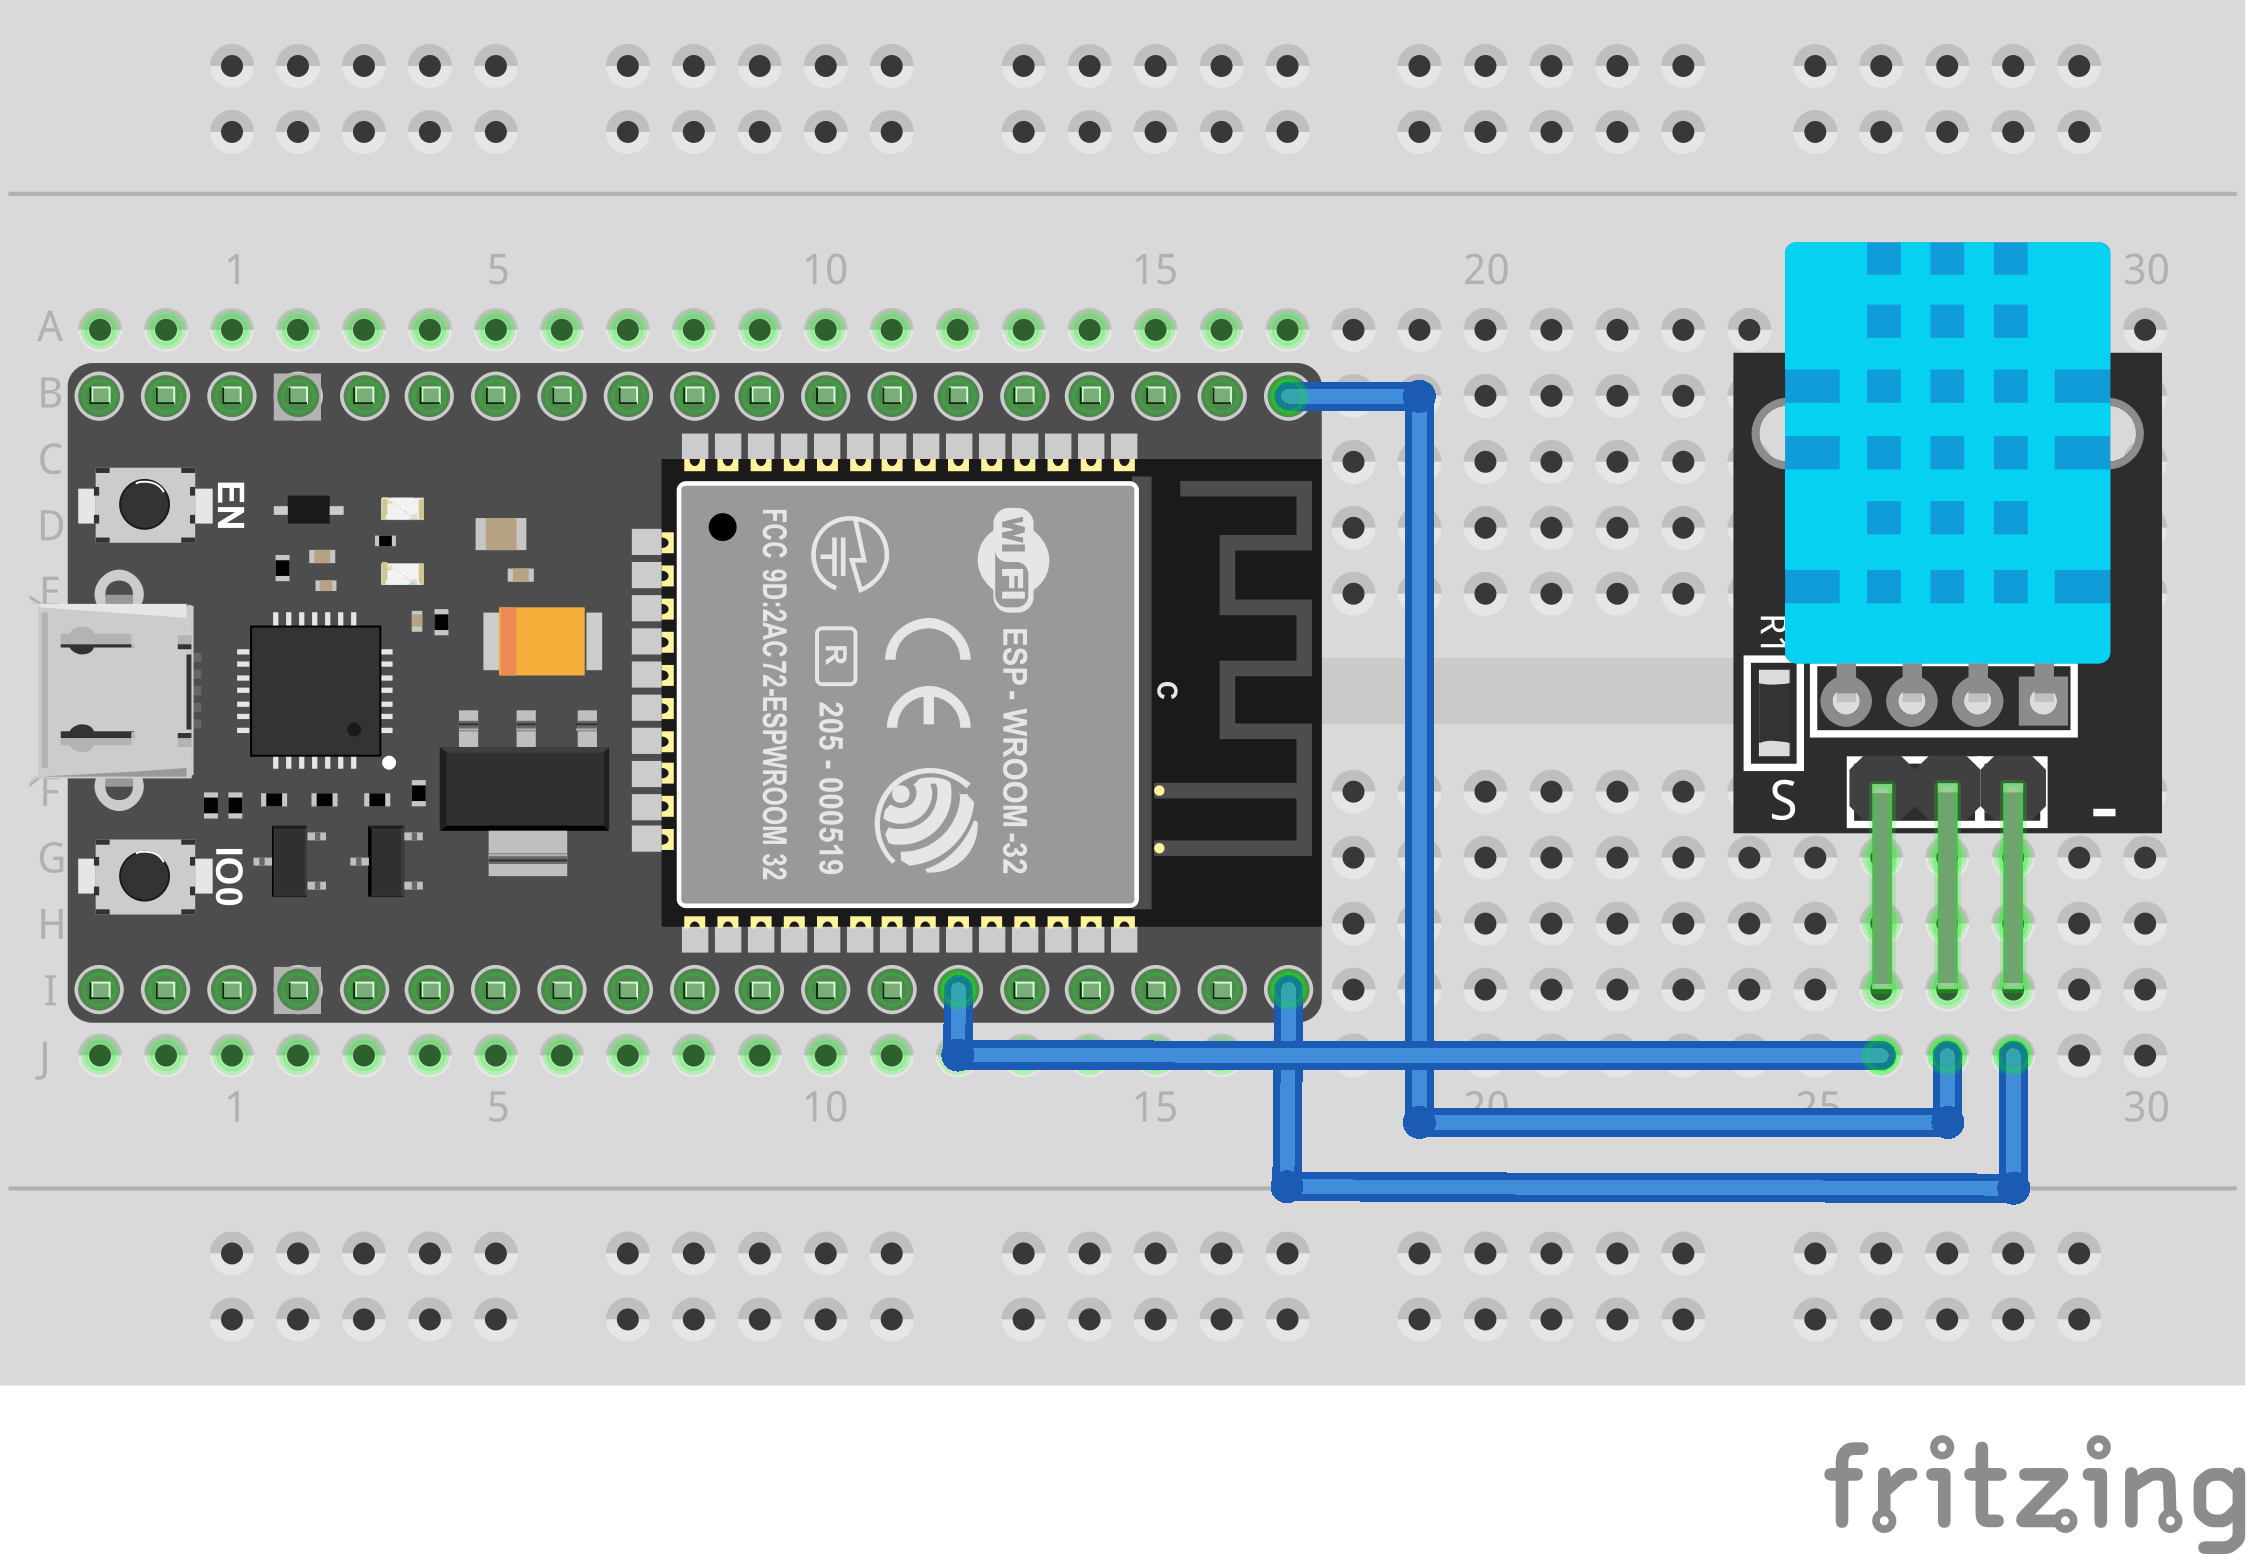
\includegraphics[width=7cm]{Artikel_bb.png}
	\caption{Aansluitingsschema tussen DHT11-sensor en ESP32 MCU.}
	\label{fig:ping}
\end{figure}

\begin{figure}[h]
	\centering
	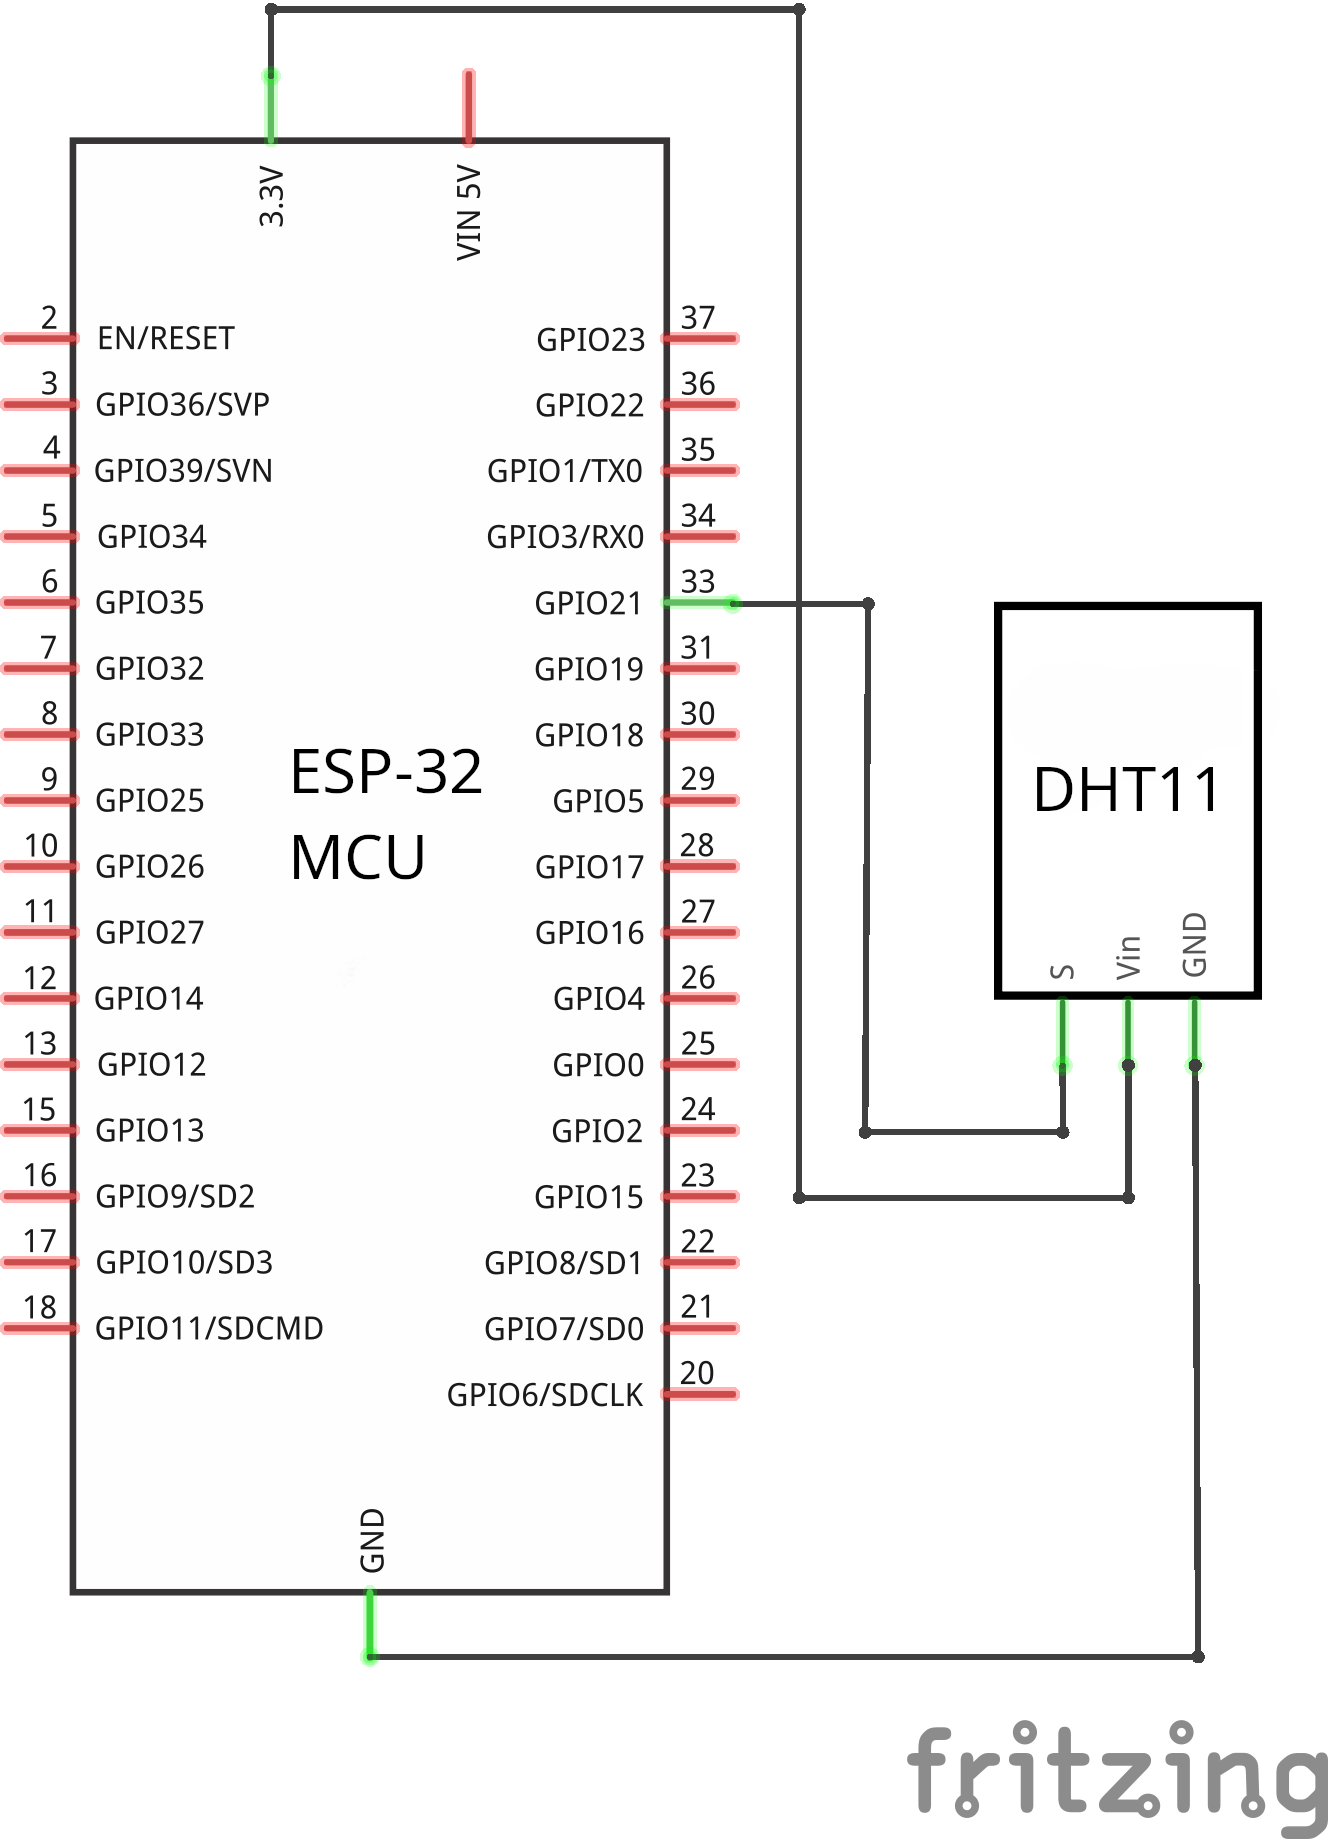
\includegraphics[width=5cm]{Artikel_schem1.png}
	\caption{Schematische weergave (CAD-tekening) tussen DHT11-sensor en ESP32 MCU}
	\label{fig:sch}
\end{figure}

\begin{figure}[h]
	\centering
	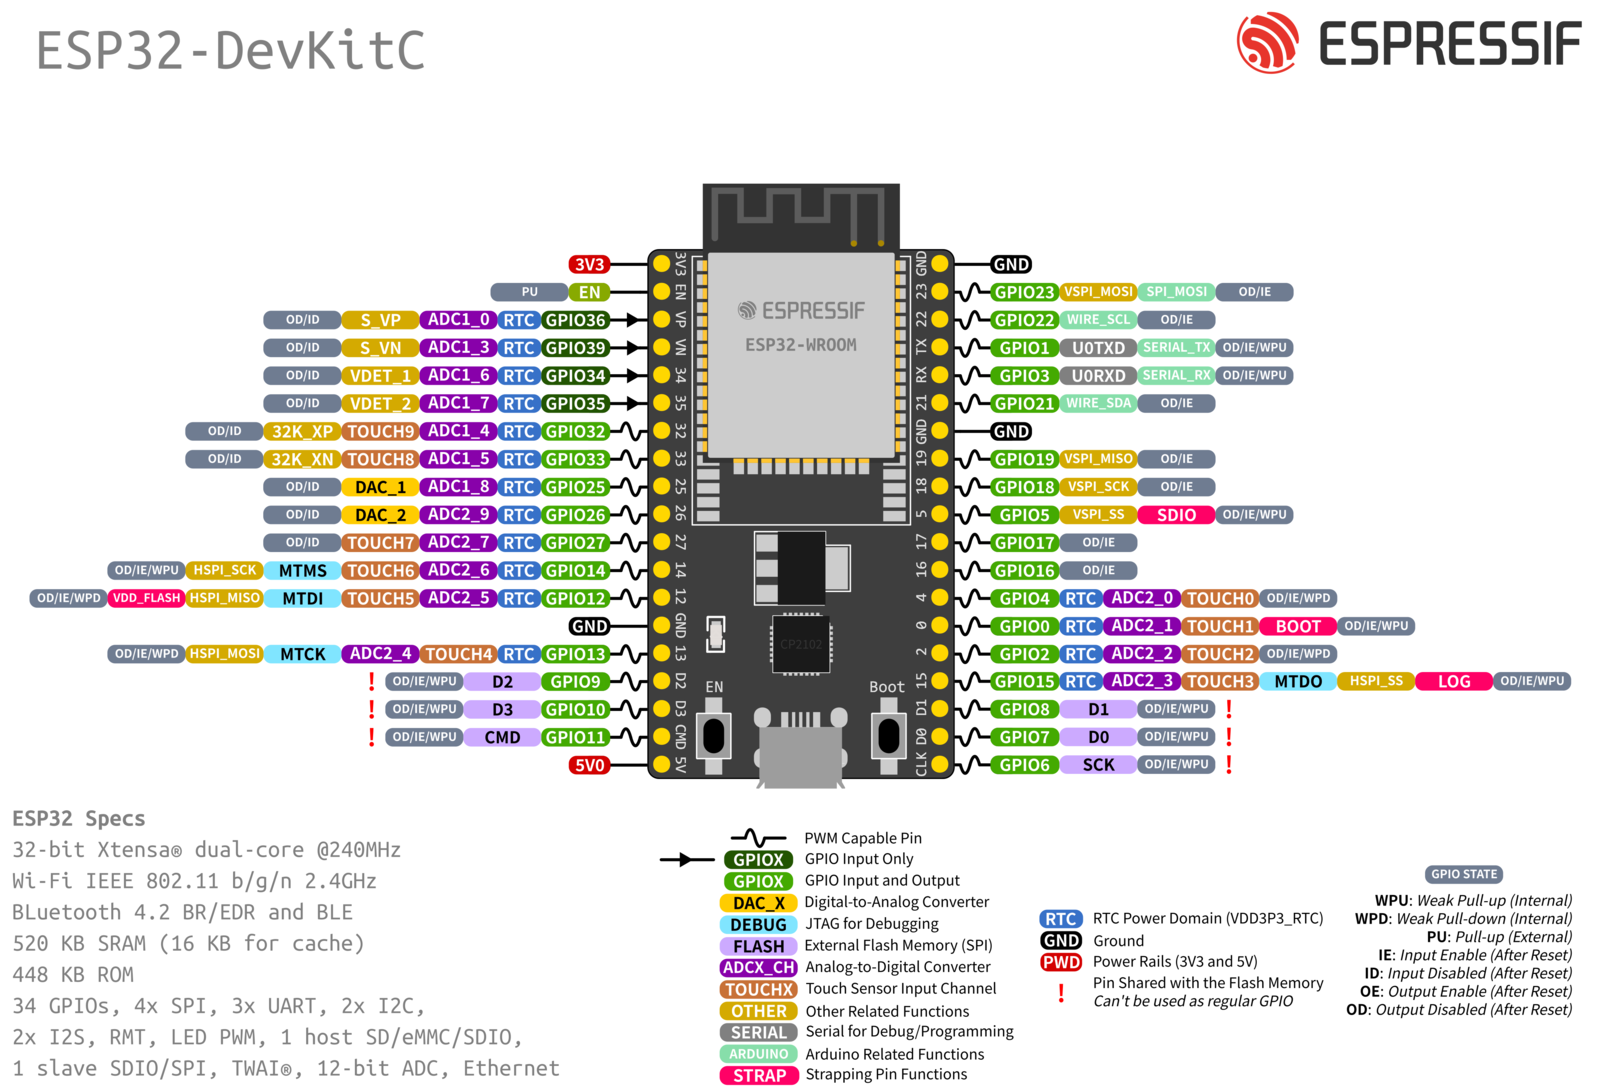
\includegraphics[width=7cm]{pinout.png}
	\caption{\textit{Pinout}-schema van ESP32 microcontroller (van datasheet).}
	\label{fig:pinout}
\end{figure}
\pagebreak
% trigger a \newpage just before the given reference
% number - used to balance the columns on the last page
% adjust value as needed - may need to be readjusted if
% the document is modified later
%\IEEEtriggeratref{8}
% The "triggered" command can be changed if desired:
%\IEEEtriggercmd{\enlargethispage{-5in}}

% references section

% can use a bibliography generated by BibTeX as a .bbl file
% BibTeX documentation can be easily obtained at:
% http://mirror.ctan.org/biblio/bibtex/contrib/doc/
% The IEEEtran BibTeX style support page is at:
% http://www.michaelshell.org/tex/ieeetran/bibtex/
\bibliography{library}{}
\bibliographystyle{IEEEtran}
% argument is your BibTeX string definitions and bibliography database(s)
%\bibliography{IEEEabrv,../bib/paper}
%
% <OR> manually copy in the resultant .bbl file
% set second argument of \begin to the number of references
% (used to reserve space for the reference number labels box)
% \begin{thebibliography}{1}

% \bibitem{IEEEhowto:kopka}
% H.~Kopka and P.~W. Daly, \emph{A Guide to \LaTeX}, 3rd~ed.\hskip 1em plus
%   0.5em minus 0.4em\relax Harlow, England: Addison-Wesley, 1999.

% \end{thebibliography}




% that's all folks
\end{document}


